\section{Der Datengenerator}\label{DerDatengenerator}
�ber den grunds�tzlichen Aufbau des Datengenerators wird im Projekt Datanbankkonfigurationen\footnote{https://dl.dropbox.com/u/608146/ADBC1\%20OLAP.pdf} eingegangen.

Um die Daten schneller in die Tabellen einzuf�gen, werden im Datengenerator die generierten Testdaten anders als in DB-Writer nicht mehr �ber Prepared Statements in die Tabellen eingef�gt, sondern �ber die write-Methode von java.io.Writer in eine Datei geschrieben. Um das umzusetzen, wurde die Komponente DB-Writer durch eine Writer-Komponente ersetzt.

Da sich auch das Data Model in diesem Projekt ge�ndert hat, m�ssen weitere Komponenten des Generators angepasst werden.
Die angepassten Komponenten des Generators zeigt Abbildung \ref{fig:KomponentendiagrammDatengenerator} auf Seite \pageref{fig:KomponentendiagrammDatengenerator}.

\begin{figure}[htp]
\centering
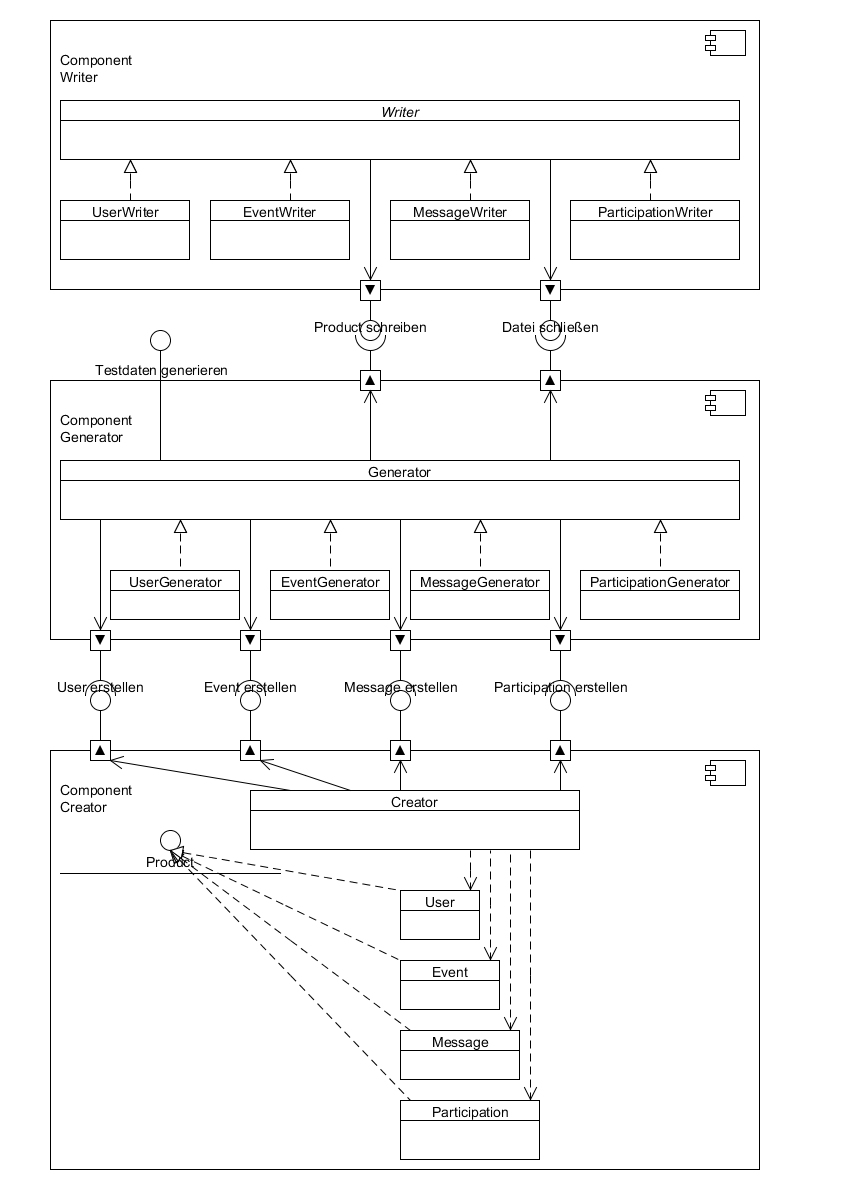
\includegraphics[width=1\textwidth]{Ingo/Bilder/Komponentendiagramm.png}
\caption{Komponentendiagramm Datengenerator}
\label{fig:KomponentendiagrammDatengenerator}
\end{figure}

Die Daten werden im CSV-Format in die jeweilige Datei geschrieben, um sie mit dem Copy-Befehl\footnote{http://www.pgadmin.org/docs/1.4/pg/sql-copy.html} von PostgreSQL in die Tabelle laden zu k�nnen.

\begin{lstlisting}[caption=COPY, firstnumber=1]{code:COPY}
COPY public.User (userId, name, email, gender, birthday, password, image) From 'C:\User.txt' DELIMITER ';'
\end{lstlisting}

Dadurch ergibt sich bei einem Umfang von 3,1 Mio generierter Zeilen im Schnitt eine Zeitersparnis um den Faktor zehn - 66 Sekunden f�r die Generierung und den Import der CSV-Datei in die Tabellen mit COPY, zu 687 Sekunden mit prepared statements.

Das Projekt liegt als Maven-Eclipse-Projekt unter:

https://github.com/rinkdotrink/ComeTogether.git